%!TEX root = nml-base.tex

\section{NML Base Schema}%
\label{s:schema}

The NML Base schema describes an information model for computer networks. 
This schema is kept intentionally general, with provisions to extend the schema to 
describe layer-specific information.

The schema consists of classes, attributes, relations, and parameters. % and logic. 
Classes describe types of objects and are described in section~\ref{sub:classes}. 
Relations describe the relations between classes and are described in section~\ref{sub:relations}. 
Attributes describe properties of classes.
% Logic describes how some relations may be derived from other relations.
Parameters, like attributes, are properties of classes, but may (subtly) change the logic.
% Logic is described in section~\ref{sub:logic}.
Attributes and parameters are described with their class description.

All classes, relations, attributes and parameters defined in this document have an 
identifier within the namespace \texttt{http://schemas.ogf.org/nml/2013/05/base\#}.

\subsection{Classes}%
\label{sub:classes}

\begin{figure}[!b]
    \centering
        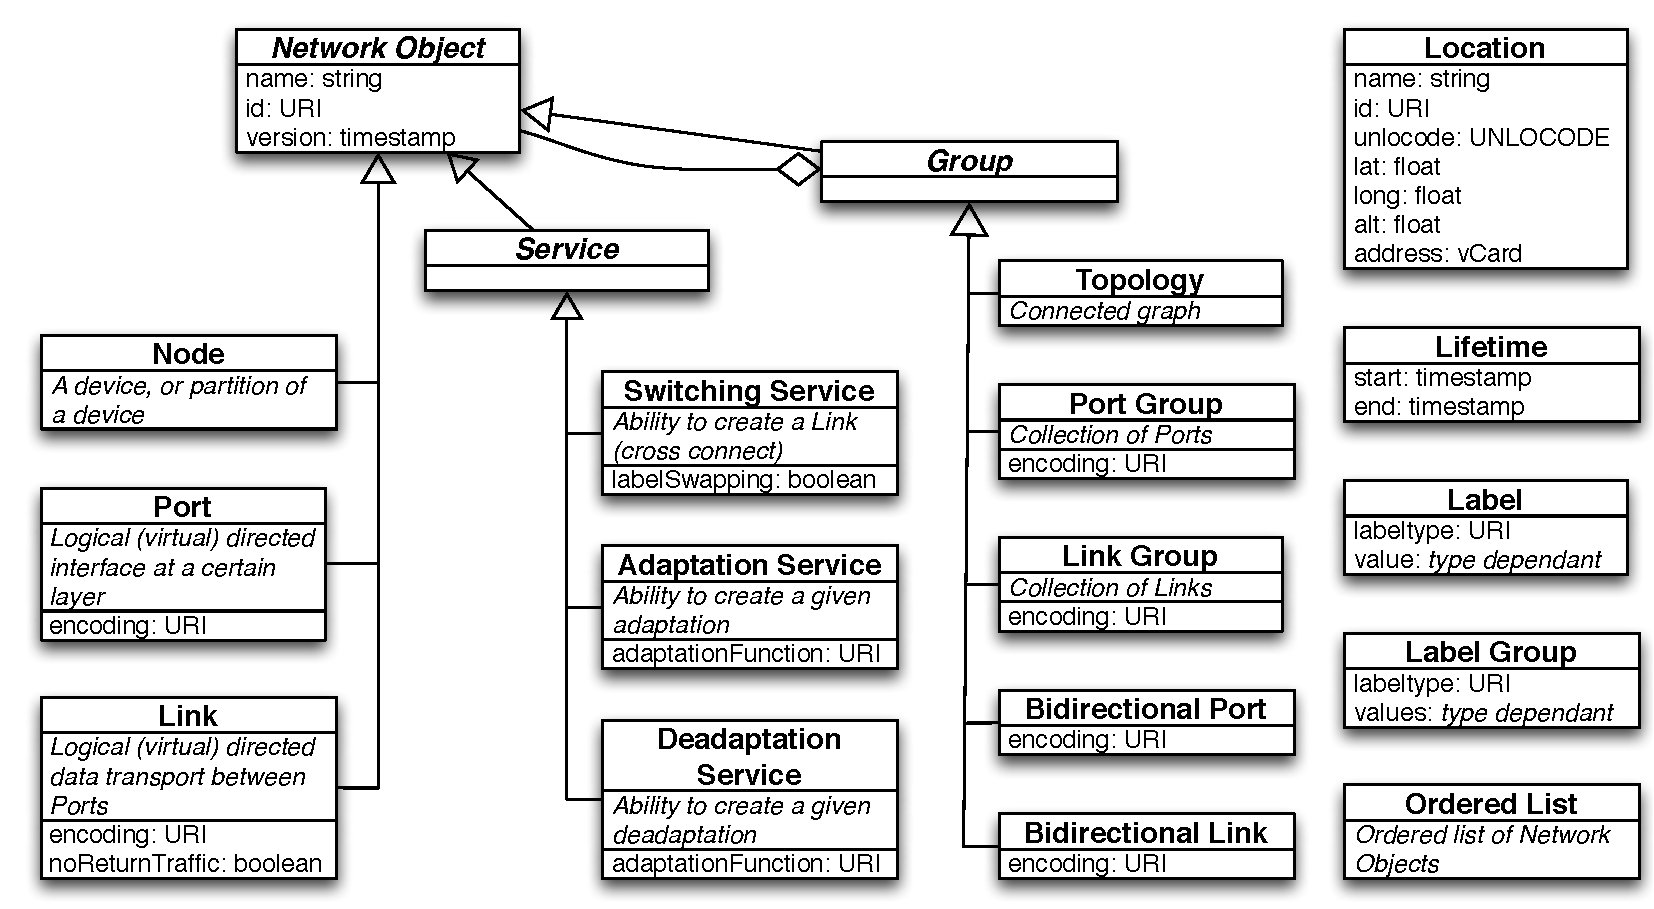
\includegraphics[width=\textwidth]{NML-hierarchy}
    \caption{A UML class diagram of the classes in the NML schema and their hierarchy}
    \label{fig:NML-schema}
\end{figure}

Figure~\ref{fig:NML-schema} shows an overview of all the classes in the NML schema in a UML class diagram. Each box defines the name of a class, a short description, and possible attributes with their value type.
%The figure also shows the relations between the objects, and their cardinalities. 
In the sections below we discuss each of the elements of the schema.

\subsubsection{Network Object}% (fold)
\label{class:network_object}

The basic abstract class of the schema is the \emph{Network Object}.  Most classes inherit from it.

\emph{Network Object} is an abstract class. It \MUSTNOT{} be instantiated directly.

A \emph{Network Object} may have the following relations:
\begin{itemize}
    \item \emph{existsDuring} to one or more \emph{Lifetime}s
    \item \emph{isAlias} to one or more \emph{Network Object}s
    \item \emph{locatedAt} to one \emph{Location} 
\end{itemize}

A \emph{Network Object} may have the following attributes:
\begin{itemize}
    \item \emph{id} to assign a persistent globally unique URI
    \item \emph{name} to assign a human readable string
    \item \emph{version} to assign a time stamp
\end{itemize}

The meaning of the \emph{isAlias} relation is only defined for specific cases (between objects of the same concrete class), and \SHOULDNOT{} be used between other objects.

The meaning of the \emph{version} attribute is only defined for specific cases (for objects of the Topology class), and \SHOULDNOT{} be used in other objects. Clients that receive a \emph{version} attribute for a non-\emph{Topology} object \SHOULD{} ignore that attribute.

An \emph{id} is a persistent, globally unique object identifier for the \emph{Network Object}. The \emph{id} \SHOULD{} be used to refer to this object. Section~\ref{s:identifiers} describes these identifiers in detail.

\emph{name} is a human readable string.
A name may be written in any language, but it is \RECOMMENDED{} that names are chosen so that all users can easily distinguish between different names. Names are not globally unique, and two objects can have the same name. It is \RECOMMENDED{} to use short, descriptive names.
A name \MUSTNOT{} be used for anything other than display purposes.  Normal Unicode recommendations apply: A name \MUSTNOT{} contain control or formatting codepoint, and it is \RECOMMENDED{} to only use codepoints from the Basic Multilingual Plane (BMP).

\emph{version} is a time stamp formatted as ISO 8601 calendar date, and \MUST{} be a basic (compact) representation with UTC timezone (\texttt{\emph{YYYYMMDD}T\emph{hhmmss}Z})~\cite{iso8601}. The time stamp can be used to publish updates of a \emph{Topology}. 
If a client receives multiple \emph{Topology} descriptions, each with a different version time stamp, the version with the latest time stamp in the past or present \MUST{} be considered the valid description. \emph{Topology} descriptions with a time stamp in the future \MAY{} be discarded or cached until the denoted time. See also the \emph{Lifetime} object to describe historic or future network changes.

The base \emph{Network Object} is subclassed into the top-level topology
components, that are sufficient to cover the description of networks.  The
classes in this schema that directly inherit from \emph{Network Object} are:

\begin{itemize}
    \item Node
    \item Port
    \item Link
    \item Service
    \item Group
\end{itemize}

These classes are described in more detail below.
% subsection network_object (end)


\subsubsection{Node}% (fold)
\label{class:node}

A \emph{Node} is generally a device connected to, or part of, the network.  A
Node does not necessarily correspond to a physical machine.

\emph{Node} inherits from \emph{Network Object}.

A \emph{Node} may have the following relations:
\begin{itemize}
    \item \emph{existsDuring} to one or more \emph{Lifetime}s
    \item \emph{hasInboundPort} to one or more \emph{Port}s or \emph{PortGroup}s
    \item \emph{hasOutboundPort} to one or more \emph{Port}s or \emph{PortGroup}s
    \item \emph{hasService} to one or more \emph{Service}s of type \emph{Switch}
    \item \emph{implementedBy} to one or more \emph{Node}s
    \item \emph{isAlias} to one or more \emph{Node}s
    \item \emph{locatedAt} to one \emph{Location} 
\end{itemize}

A \emph{Node} may have the following attributes:
\begin{itemize}
    \item \emph{id} to assign a persistent globally unique URI
    \item \emph{name} to assign a human readable string
\end{itemize}

% subsection node (end)


\subsubsection{Port}% (fold)
\label{class:port}

A \emph{Port} defines connectivity from a \emph{Network Object} to the rest of the network. A \emph{Port} object is unidirectional. A \emph{Port} does not necessarily correspond to a physical interface. It represents a logical transport entity at a fixed place in the network.

\emph{Port} inherits from \emph{Network Object}.

A \emph{Port} may have the following relations:
\begin{itemize}
    \item \emph{existsDuring} to one or more \emph{Lifetime}s
    \item \emph{hasLabel} to one \emph{Label}
    \item \emph{hasService} to one or more \emph{Service}s of type \emph{Adaptation} or type \emph{Deadaptation}
    \item \emph{isAlias} to one or more \emph{Port}s
    \item \emph{isSink} to one or more \emph{Link}s
    \item \emph{isSource} to one or more \emph{Link}s
\end{itemize}

A \emph{Port} may have the following attributes:
\begin{itemize}
    \item \emph{encoding} to assign a data encoding identifier
    \item \emph{id} to assign a persistent globally unique URI
    \item \emph{name} to assign a human readable string
\end{itemize}

The \emph{encoding} attribute defines the format of the data streaming through the Port. The identifier for the encoding \MUST{} be a URI. Encoding URIs \SHOULD{} be specified in a Grid Forum Documents (GFD).
% subsection port (end)


\subsubsection{Link}% (fold)
\label{class:link}

A \emph{Link} object describes a unidirectional data transport from each of its sources to all of its sinks.

A source of a Link is a Network Object, e.g.\ a \emph{Port}, that has a \emph{isSource} relation to the \emph{Link}.
A sink of a Link is a Network Object, e.g.\ a \emph{Port}, that has a \emph{isSink} relation to the \emph{Link}.

A \emph{Link} object can refer to any link connection. A link segment and an end-to-end path are both described by a \emph{Link} object. The composition of links into a path, and decomposition into link segments is described by the \emph{isSerialCompoundLink} relation.

\emph{Link} inherits from \emph{Network Object}.

A \emph{Link} may have the following relations:
\begin{itemize}
    \item \emph{existsDuring} to one or more \emph{Lifetime}s
    \item \emph{hasLabel} to one \emph{Label}
    \item \emph{isAlias} to one or more \emph{Link}s
    \item \emph{isSerialCompoundLink} to one \emph{Ordered List} of \emph{Link}s
\end{itemize}

A \emph{Link} may have the following attributes:
\begin{itemize}
    \item \emph{encoding} to assign a data encoding identifier
    \item \emph{id} to assign a persistent globally unique URI
    \item \emph{name} to assign a human readable string
\end{itemize}

A \emph{Link} may have the following parameter:
\begin{itemize}
    \item \emph{noReturnTraffic}. A value of \texttt{true} changes the definition of \emph{Link} to: data transport from each sources to all sinks, except that there is no data transport from a source to a sink if the source and sink are grouped together in a \emph{BidirectionalPort} group. The default value of \emph{noReturnTraffic} is \texttt{false}.
    
    An example of where this is used is in an Ethernet broadcast domain, where broadcast traffic is sent to all sinks, except the sink \emph{Port}s associated with the sending source \emph{Port}.
\end{itemize}

The \emph{encoding} attribute defines the format of the data streaming through the \emph{Link}. The identifier for the encoding \MUST{} be a URI. Encoding URIs \SHOULD{} be specified in a Grid Forum Documents (GFD).
% subsection link (end)


\subsubsection{Service}% (fold)
\label{class:service}

\emph{Service} describes an ability of the network. That is, it describes how the behavior can be changed dynamically.

\emph{Service} is an abstract class. It \MUSTNOT{} be instantiated directly.

\emph{Service} inherits from \emph{Network Object}.
A \emph{Service} may have the same relations, attributes and parameters as a \emph{Network Object}.

This schema defines three different services, the \emph{SwitchingService} the \emph{AdaptationService} and the \emph{DeadaptationService}. These are described in more detail below. 
% subsection service (end)


\subsubsection{Switching Service}% (fold)
\label{class:switching_service}

A \emph{SwitchingService} describes the ability to create new \emph{Link}s from any of its inbound \emph{Port}s to any of its outbound \emph{Port}s.

\emph{SwitchingService} inherits from \emph{Service}.

A \emph{SwitchingService} may have the following relations:
\begin{itemize}
    \item \emph{encoding} to assign a data encoding identifier
    \item \emph{existsDuring} to one or more \emph{Lifetime}s
    \item \emph{hasInboundPort} to one or more \emph{Port}s or \emph{PortGroup}s
    \item \emph{hasOutboundPort} to one or more \emph{Port}s or \emph{PortGroup}s
    \item \emph{isAlias} to one or more \emph{Switching Service}s
    \item \emph{providesLink} to one or more \emph{Link}s or \emph{LinkGroup}s.
\end{itemize}

A \emph{SwitchingService} may have the following attributes:
\begin{itemize}
    \item \emph{id} to assign a persistent globally unique URI
    \item \emph{name} to assign a human readable string
\end{itemize}

A \emph{SwitchingService} may have the following parameter:
\begin{itemize}
    \item \emph{labelSwapping}. A value of \texttt{false} adds a restriction to the \emph{SwitchingService}: it is only able to create cross connects from an inbound \emph{Port} to an outbound \emph{Port} if the \emph{Label} of the connected \emph{Port}s have the same value. The default value is \texttt{false}.
\end{itemize}

The \emph{providesLink} relation points to \emph{Link}s which describe the currently configured cross connects in a \emph{SwitchingService}.

A \emph{Port} object can have a \emph{hasService} relation, however the \emph{SwitchingService} defines a more specific relation \emph{hasInboundPort} / \emph{hasOutboundPort} relation to a \emph{Port} object. The latter relation is preferred over the \emph{hasService} relation of the Port to the SwitchingService.

The \emph{encoding} attribute defines the format of the data streaming through the \emph{SwitchingService}. The identifier for the encoding \MUST{} be a URI. Encoding URIs \SHOULD{} be specified in a Grid Forum Documents (GFD).
% subsection switching_service (end)


\subsubsection{Adaptation Service}% (fold)
\label{class:adaptation_service}

An \emph{AdaptationService} describes the ability that data from one or more \emph{Port}s can be embedded in the data encoding of one other \emph{Port}. This is commonly referred to as the embedding of client layer (higher network layer) ports in a server layer (lower network layer) port. The \emph{AdaptationService} describes a multiplexing adaptation function, meaning that different channels (the client layer ports) can be embedded in a single data stream (the server layer port). For example multiplexing several VLANs over a single trunk port.

Like \emph{Port} and \emph{Link}, \emph{AdaptationService} describes a unidirectional transport function. For the inverse transport function, see \emph{DeadaptationService}.

\emph{AdaptationService} inherits from \emph{Service}.

An \emph{AdaptationService} may have the following relations:
\begin{itemize}
    \item \emph{canProvidePort} to one or more \emph{Port}s or \emph{PortGroup}s (this describes a ability)
    \item \emph{existsDuring} to one or more \emph{Lifetime}s
    \item \emph{isAlias} to one or more \emph{AdaptationService}s
    \item \emph{providesPort} to one or more \emph{Port}s or \emph{PortGroup}s (this describes a configuration)
\end{itemize}

An \emph{AdaptationService} may have the following attributes:
\begin{itemize}
    \item \emph{adaptationFunction} to assign an adaptation technology identifier
    \item \emph{id} to assign a persistent globally unique URI
    \item \emph{name} to assign a human readable string
\end{itemize}

\emph{DeadaptationService} is an inverse of \emph{AdaptationService}. This should not be confused with an inverse multiplexing adaptation function. An inverse multiplexing adaptation function embeds a single data stream in multiple underlying data streams. To describes such a network, the \emph{parallelCompound} relation can be used, which is a future extension relation, described in a separate document~\cite{nml-experimental}.

% subsection adaptation_service (end)


\subsubsection{De-adaptation Service}% (fold)
\label{class:deadaptation_service}

A \emph{DeadaptationService} describes the ability that data of one or more ports can be extracted from the data encoding of one other port. This is commonly referred to as the extraction of client layer (higher network layer) ports from the server layer (lower network layer) port. The \emph{DeadaptationService} describes a demultiplexing adaptation function, meaning that different channels (the client layer ports) can be extracted from a single data stream (the server layer port). For example demultiplexing several VLANs from a single trunk port.

Like \emph{Port} and \emph{Link}, \emph{AdaptationService} describes a unidirectional transport function. For the inverse transport function, see \emph{AdaptationService}.%

\emph{DeadaptationService} inherits from \emph{Service}.

A \emph{DeadaptationService} may have the following relations:
\begin{itemize}
    \item \emph{canProvidePort} to one or more \emph{Port}s or \emph{PortGroup}s
    \item \emph{existsDuring} to one or more \emph{Lifetime}s
    \item \emph{isAlias} to one or more \emph{DeadaptationService}s
    \item \emph{providesPort} to one or more \emph{Port}s or \emph{PortGroup}s
\end{itemize}

A \emph{DeadaptationService} may have the following attributes:
\begin{itemize}
    \item \emph{adaptationFunction} to assign a adaptation technology identifier
    \item \emph{id} to assign a persistent globally unique URI
    \item \emph{name} to assign a human readable string
\end{itemize}

% subsubsection adaptation_service (end)


\subsubsection{Group}% (fold)
\label{class:group}

A \emph{Group} describes a collections of objects. Any object can be part of a group, including another \emph{Group}. An object can also be part of multiple \emph{Group}s.

\emph{Group} is an abstract class. It \MUSTNOT{} be instantiated directly.

\emph{Group} inherits from \emph{Network Object}.
A \emph{Group} may have the same relations, attributes and parameters as a \emph{Network Object}.

This schema defines five different \emph{Group}s:

\begin{itemize}
    \item Topology
    \item Port Group
    \item Link Group
    \item Bidirectional Port
    \item Bidirectional Link
\end{itemize}

These classes are described in more detail below.
% subsubsection group (end)



\subsubsection{Topology}% (fold)
\label{class:topology}

A \emph{Topology}\footnote{At first this was called a Network, then Graph Network. The term Topology was suggested to avoid the confusion surrounding the overloaded term Network.} is a set of connected \emph{Network Object}s. \emph{connected} means that there is, or it is possible to create, a data transport between any two Network Objects in the same Topology, provided that there are no policy, availability or technical restrictions.

A \emph{Topology} may have the following relations:
\begin{itemize}
    \item \emph{existsDuring} to one or more \emph{Lifetime}s
    \item \emph{hasNode} to one or more \emph{Node}s
    \item \emph{hasInboundPort} to one or more \emph{Port}s or \emph{PortGroup}s
    \item \emph{hasOutboundPort} to one or more \emph{Port}s or \emph{PortGroup}s
    \item \emph{hasService} to one or more \emph{Service} of type \emph{Switch}
    \item \emph{hasTopology} to one or more \emph{Topology}s
    \item \emph{isAlias} to one or more \emph{Topology}s
    \item \emph{locatedAt} to one \emph{Location} 
\end{itemize}

A \emph{Topology} may have the following attributes:
\begin{itemize}
    \item \emph{id} to assign a persistent globally unique URI
    \item \emph{name} to assign a human readable string
    \item \emph{version} to assign a serial number
\end{itemize}

The \emph{version} attribute is described at the \emph{Network Object}.
% subsubsection topology (end)


\subsubsection{Port Group}% (fold)
\label{class:port_group}

A \emph{PortGroup} is an unordered set of \emph{Port}s.

A \emph{PortGroup} may have the following relations:
\begin{itemize}
    \item \emph{existsDuring} to one or more \emph{Lifetime}s
    \item \emph{hasLabelGroup} to one \emph{LabelGroup}
    \item \emph{hasPort} to one or more \emph{Port}s or \emph{PortGroups}
    % \item \emph{hasService} to one or more \emph{Service}s of type Adaptation or type Deadaptation
    \item \emph{isAlias} to one or more \emph{PortGroup}s
    \item \emph{isSink} to one or more \emph{LinkGroup}s
    \item \emph{isSource} to one or more \emph{LinkGroup}s
\end{itemize}

A \emph{PortGroup} may have the following attributes:
\begin{itemize}
    \item \emph{encoding} to assign a data encoding identifier
    \item \emph{id} to assign a persistent globally unique URI
    \item \emph{name} to assign a human readable string
\end{itemize}

% subsubsection port_group (end)


\subsubsection{Link Group}% (fold)
\label{class:link_group}

A \emph{LinkGroup} is an unordered set of \emph{Link}s.

A \emph{LinkGroup} may have the following relations:
\begin{itemize}
    \item \emph{existsDuring} to one or more \emph{Lifetime}s
    \item \emph{hasLabelGroup} to one \emph{LabelGroup}
    \item \emph{hasLink} to one or more \emph{Link}s or \emph{LinkGroup}s
    \item \emph{isAlias} to one or more \emph{LinkGroup}s
    \item \emph{isSerialCompoundLink} to \emph{Ordered List} of \emph{LinkGroup}s
\end{itemize}

A \emph{LinkGroup} may have the following attributes:
\begin{itemize}
    \item \emph{id} to assign a persistent globally unique URI
    \item \emph{name} to assign a human readable string
\end{itemize}

% subsubsection link_group (end)


\subsubsection{Bidirectional Port}% (fold)
\label{class:bidirectional_port}

A \emph{BidirectionalPort} is a group of two (unidirectional) 
\emph{Port}s or \emph{PortGroup}s together forming a bidirectional representation of a physical or 
virtual port. See Figure~\ref{fig:Port-Link} for an example of a \emph{BidirectionalPort} and its associated \emph{Port}s.

A \emph{BidirectionalPort} may have the following relations:
\begin{itemize}
    \item \emph{existsDuring} to one or more \emph{Lifetime}s
    \item \emph{hasPort} to exactly two \emph{Port}s or two \emph{PortGroup}s
\end{itemize}

A \emph{BidirectionalPort} may have the following attributes:
\begin{itemize}
    \item \emph{encoding} to assign a data encoding identifier
    \item \emph{id} to assign a persistent globally unique URI
    \item \emph{name} to assign a human readable string
\end{itemize}

There is explicitly no direct relation between a \emph{BidirectionalPort} and a \emph{BidirectionalLink}, since NML is a unidirectional model.
% subsubsection bidirectional_port (end)

\begin{figure}[htbp]
    \centering
        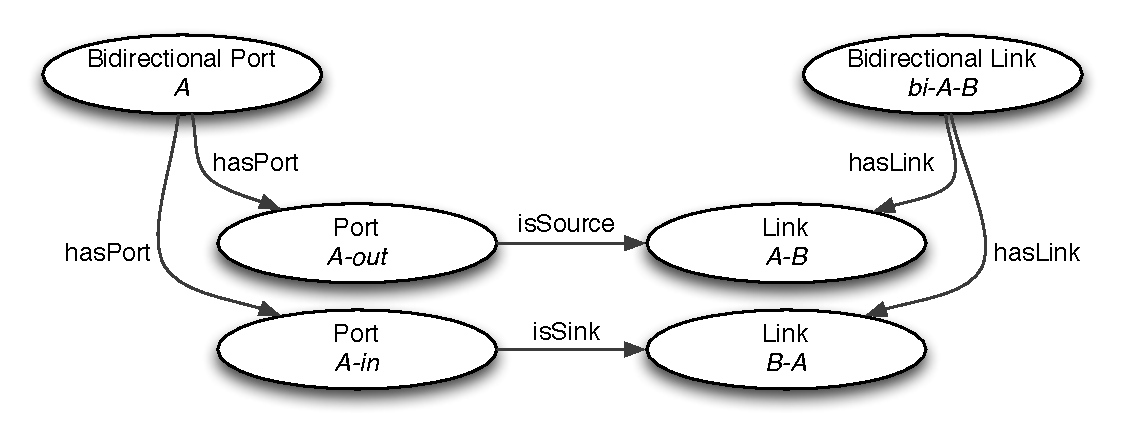
\includegraphics[width=.8\textwidth]{Port-Link.pdf}
    \caption{An abstract example of \emph{BidirectionalPort} and \emph{BidirectionalLink}}
    \label{fig:Port-Link}
\end{figure}


\subsubsection{Bidirectional Link}% (fold)
\label{class:bidirectional_link}

A \emph{BidirectionalLink} is a group of two (unidirectional) \emph{Link}s or \emph{LinkGroup}s together forming a bidirectional link. See Figure~\ref{fig:Port-Link} for an example of a \emph{BidirectionalLink} and its associated \emph{Link}s.

A \emph{BidirectionalLink} may have the following relations:
\begin{itemize}
    \item \emph{existsDuring} to one or more \emph{Lifetime}s
    \item \emph{hasLink} to exactly two \emph{Link}s or two \emph{LinkGroup}s
\end{itemize}

A \emph{BidirectionalLink} may have the following attributes:
\begin{itemize}
    \item \emph{encoding} to assign a data encoding identifier
    \item \emph{id} to assign a persistent globally unique URI
    \item \emph{name} to assign a human readable string
\end{itemize}

There is explicitly no direct relation between a \emph{BidirectionalPort} and a \emph{BidirectionalLink}, since NML is a unidirectional model.
% subsubsection bidirectional_link (end)


\subsubsection{Location}% (fold)
\label{class:location}

A \emph{Location} is a reference to a geographical location or area. A \emph{Location} object can be related to other \emph{Network Object}s to describe that these are located there. This can be relevant for network measurements, visualisations, et cetera.

A \emph{Location} may have the following attributes:
\begin{itemize}
    \item \emph{id} to assign a persistent globally unique URI
    \item \emph{name} to assign a human readable string
    \item \emph{long} is the longitude in WGS84 coordinate system (in decimal degrees)~\cite{wgs84}
    \item \emph{lat} is the latitude in WGS84 coordinate system (in decimal degrees)
    \item \emph{alt} is the altitude in WGS84 coordinate system (in decimal meters) 
    \item \emph{unlocode} is the UN/LOCODE location identifier~\cite{unlocode}
    \item \emph{address} is a vCard ADR (address) property. The exact syntax of the address property is not specified, to allow other (e.g.\ XML or RDF) representations of the string-based format specified in \cite{vcard}.
\end{itemize}

% subsubsection location (end)


\subsubsection{Lifetime}% (fold)
\label{class:lifetime}

A \emph{Lifetime} is an interval between which the object is said to be active. This can be used to track changes in a network, reflect dynamic operations, to help debug problems, et cetera.

A \emph{Lifetime} \MAY{} have the following attributes:
\begin{itemize}
    \item \emph{start} is the start time and date formatted as ISO 8601 calendar date, and \SHOULD{} be a basic (compact) representation with UTC timezone (\texttt{\emph{YYYYMMDD}T\emph{hhmmss}Z})~\cite{iso8601}
    \item \emph{end} is the end time and date formatted as ISO 8601 calendar date, and \SHOULD{} be a basic (compact) representation with UTC timezone (\texttt{\emph{YYYYMMDD}T\emph{hhmmss}Z})
\end{itemize}

Objects with multiple lifetimes mean that the lifetime of the object is the union of all lifetimes (as opposed to a intersection).

If a Network Object has no associated \emph{Lifetime} objects, or the start or end attribute of a Lifetime object is missing, the default lifetime may be assumed to start on or before the time specified in the version attribute of the most specific Topology object that contains this Network Object. The end of that assumed lifetime is indefinite, until a Topology object with a higher version number is published. This new description can define a new Lifetime for the object, or the Topology. If the new description does not contain the Network Object, the end time is assumed to have passed.

If a Network Object has no associated Lifetime objects, and the Topology object does not have a version attribute, than the lifetime of the Network Object is undefined.

% subsubsection lifetime (end)


\subsubsection{Label}% (fold)
\label{class:label}

A \emph{Label} is the technology-specific value that distinguishes a single data stream (a channel) embedded in a larger data stream. The \emph{Label} can be a resource label (with one value). In a future extension it may be a pair of source and destination labels (with two values)~\cite{g800}. Examples of resource labels are a VLAN number, wavelength, et cetera.

A \emph{Label} may have the following attributes:
\begin{itemize}
    \item \emph{labeltype} to refer to a technology-specific labelset, e.g.\ a URI for VLANs
    \item \emph{value} is one specific value taken from the labelset, e.g.\ a VLAN number
\end{itemize}

Technology extensions of NML may define additional attributes. Label type URIs \SHOULD{} be specified in a Grid Forum Documents (GFD), which \SHOULD{} also define possible values.

This version of NML only deals with resource labels. The use of source and destination labels is a future extension~\cite{nml-experimental}.


% subsubsection label (end)


\subsubsection{Label Group}% (fold)
\label{class:label_group}

A \emph{LabelGroup} is an unordered set of \emph{Label}s.

A \emph{LabelGroup} may have the following attributes:
\begin{itemize}
    \item \emph{labeltype} to refer to a technology-specific labelset
    \item \emph{values} is a set of specific values taken from the labelset
\end{itemize}

Technology extensions of NML may define additional attributes.
% subsubsection label_group (end)


\subsubsection{Ordered List}% (fold)
\label{class:ordered_list}

An \emph{Ordered List} is an ordered list of \emph{Network Object}s. These are used for the \emph{isSerialCompoundLink} relation to an ordered list of \emph{Link}s to describe a path through the network.

The representation of an \emph{Ordered List} depends on the syntax, and is defined in section~\ref{sub:ordered_lists}.
% subsubsection ordered_list (end)


\subsubsection{List Item}% (fold)
\label{class:list_item}

A \emph{ListItem} is a syntactical construct which may be used by syntaxes to construct a \emph{Ordered List}. The exact usage depends on the syntax.
% subsubsection list_item (end)



\subsection{Relations}
\label{sub:relations}

\emph{Relation}s describe how different \emph{Network Object}s relate to each other, 
typically to form a network topology description. 
The relations have been listed above, and are defined here (in alphabetical order). 
In principle a \emph{Relation} can go from any object to any other object. 

The list below makes a distinction between \emph{allowed} and \emph{defined} relations.
An \emph{allowed} relation means it is valid NML.
A \emph{defined} relation means that it has a specific meaning, as described here.

A relation which is \textsc{not} \emph{allowed} \MUST{} be rejected by a client, and the sender \SHOULD{} be notified with an error.
A relation which is \emph{allowed}, but (yet) \emph{undefined} \SHOULD{} be ignored by a client (either silently, or with a warning to the sender).
This distinction allows future extension of NML, while retaining limited backward compatibility.

The \emph{existsDuring}, \emph{hasLabel}, \emph{hasLabelGroup}, \emph{hasLink}, 
\emph{hasNode}, \emph{hasPort}, \emph{hasService}, \emph{hasTopology}, 
\emph{locatedAt}, \emph{providesLink}, and \emph{providesPort} are defined as 
\emph{implicit} relations. All other relations are \emph{explicit}. 
The distinction between implicit and explicit relations may be used by a syntax to 
allow a more compact network description.

\subsubsection{canProvidePort}% (fold)
\label{rel:canProvidePort}

\emph{canProvidePort} is used to relate an \emph{AdaptationService} or 
\emph{DeadaptationService} to one or more \emph{Port}s or \emph{PortGroup}s 
to define that these can be created by that \emph{AdaptationService} or 
\emph{DeadaptationService}.

Allowed relations are:
\begin{itemize}
    \item \nmlrelation{Service}{*}{canProvidePort}{*}{Port}
    \item \nmlrelation{Service}{*}{canProvidePort}{*}{PortGroup}
\end{itemize}

Defined relations are:
\begin{itemize}
    \item \nmlrelation{AdaptationService}{*}{canProvidePort}{*}{Port}
    \item \nmlrelation{AdaptationService}{*}{canProvidePort}{*}{PortGroup}
    \item \nmlrelation{DeadaptationService}{*}{canProvidePort}{*}{Port}
    \item \nmlrelation{DeadaptationService}{*}{canProvidePort}{*}{PortGroup}
\end{itemize}

\subsubsection{existsDuring}% (fold)
\label{rel:existsDuring}

\emph{existsDuring} relates one \emph{Network Object} object to zero or more \emph{LifeTime} objects. This defines the existence of the object at a certain time.

\nmlrelation{Network Object}{1}{existsDuring}{*}{LifeTime}

Objects with multiple lifetimes mean that the lifetime of the object is the union of all lifetimes (as opposed to a intersection).

If a Network Object has no associated Lifetime objects, or the start or end attribute of a Lifetime object is missing, the default lifetime may be assumed to start on or before the time specified in the version attribute of the most specific Topology object that contains this Network Object, and the end on or later than the version attribute of the next published Topology object.

If a Network Object has no associated Lifetime objects, and the Topology object does not have a version attribute, then the lifetime of the Network Object is undefined.

\subsubsection{hasInboundPort}% (fold)
\label{rel:hasInboundPort}

\emph{hasInboundPort} defines the relation between a \emph{Node}, a \emph{SwitchingService} or a \emph{Topology} and their respective \emph{Port}s or \emph{PortGroup}s

Allowed relations are:
\begin{itemize}
    \item \nmlrelation{Network Object}{*}{hasInboundPort}{*}{Port}
    \item \nmlrelation{Network Object}{*}{hasInboundPort}{*}{PortGroup}
\end{itemize}

Defined relations are:
\begin{itemize}
    \item \nmlrelation{Node}{*}{hasInboundPort}{*}{Port}
    \item \nmlrelation{Node}{*}{hasInboundPort}{*}{PortGroup}
    \item \nmlrelation{SwitchingService}{*}{hasInboundPort}{*}{Port}
    \item \nmlrelation{SwitchingService}{*}{hasInboundPort}{*}{PortGroup}
    \item \nmlrelation{Topology}{*}{hasInboundPort}{*}{Port}
    \item \nmlrelation{Topology}{*}{hasInboundPort}{*}{PortGroup}
\end{itemize}

This defines that the related \emph{Network Object} has an inbound \emph{Port} or \emph{PortGroup} object. The direction of the \emph{Port} object is relative to the \emph{Network Object} the \emph{Port} is attached to, so in this case the traffic flows towards that \emph{Network Object} (similarly for the \emph{PortGroup}). This \emph{Port} would then be related to a \emph{Link} object using the \emph{isSink} relation (or a \emph{PortGroup} and \emph{LinkGroup} respectively).

A \emph{Network Object} with a \emph{hasInboundPort} relation pointing to a \emph{PortGroup} has the same meaning as defining a \emph{hasInboundPort} relation pointing to every \emph{Port} in that \emph{PortGroup} (as defined by a \emph{hasPort} relation between the \emph{PortGroup} and \emph{Port}).


\subsubsection{hasLabel}% (fold)
\label{rel:hasLabel}

\emph{hasLabel} assigns one \emph{Label} to a \emph{Port} or \emph{Link}

Allowed relations are:
\begin{itemize}
    \item \nmlrelation{Port}{1}{hasLabel}{*}{Label}
    \item \nmlrelation{Link}{1}{hasLabel}{*}{Label}
\end{itemize}

The \emph{Label} assigned to a \emph{Port} or \emph{Link} is the technology label that identifies the traffic through this \emph{Port} or \emph{Link} (including in \emph{Link}s provided by a \emph{SwitchingMatrix}).

A \emph{Label} is used to distinguish a \emph{Port} in a \emph{PortGroup}, or distinguish a \emph{Link} in a \emph{LinkGroup}.

The meaning of \emph{hasLabel} is only \emph{defined} for a cardinality of 0 or 1.


\subsubsection{hasLabelGroup}% (fold)
\label{rel:hasLabelGroup}

\emph{hasLabelGroup} assigns one \emph{LabelGroup} to a \emph{PortGroup} or \emph{LinkGroup}

Allowed relations are:
\begin{itemize}
    \item \nmlrelation{PortGroup}{1}{hasLabelGroup}{*}{LabelGroup}
    \item \nmlrelation{LinkGroup}{1}{hasLabelGroup}{*}{LabelGroup}
\end{itemize}

The \emph{LabelGroup} assigned to this \emph{PortGroup} or \emph{LinkGroup} defines the \emph{Label}s associated with the \emph{Port}s member of that group. There  \MUST{} be a one-to-one correspondence between the \emph{LabelGroup} and the \emph{PortGroup}.

The meaning of \emph{hasLabelGroup} is only defined for a cardinality of 0 or 1.

\subsubsection{hasLink}% (fold)
\label{rel:hasLink}

\emph{hasLink} is used for:
    \begin{itemize}
        \item \emph{BidirectionalLink} to relate exactly two \emph{Link}s or two \emph{LinkGroup}s
        \item \emph{LinkGroup} to one or more \emph{Link}s or \emph{LinkGroup}s to define membership of that group
    \end{itemize}

Allowed relations are:
\begin{itemize}
    \item \nmlrelation{Group}{*}{hasLink}{*}{Link}
    \item \nmlrelation{Group}{*}{hasLink}{*}{LinkGroup}
\end{itemize}

Defined relations are:
\begin{itemize}
    \item \nmlrelation{LinkGroup}{*}{hasLink}{*}{Link}
    \item \nmlrelation{LinkGroup}{*}{hasLink}{*}{LinkGroup}
    \item \nmlrelation{BidirectionalLink}{*}{hasLink}{2}{Link}
    \item \nmlrelation{BidirectionalLink}{*}{hasLink}{2}{LinkGroup}
\end{itemize}

The \emph{hasLink} relationships for a \emph{BidirectionalLink} point to the two unidirectional \emph{Link}s that together form a bidirectional connection between its respective associated \emph{Node}s.

The \emph{hasLink} relationships for a \emph{LinkGroup} define the membership of the \emph{Link}s in that \emph{LinkGroup}.

\subsubsection{hasNode}% (fold)
\label{rel:hasNode}

\emph{hasNode} relates a \emph{Topology} to a \emph{Node}, meaning that a \emph{Node} is part of a \emph{Topology}

Allowed relations are:
\begin{itemize}
    \item \nmlrelation{Network Object}{*}{hasNode}{*}{Node}
\end{itemize}

Defined relations are:
\begin{itemize}
    \item \nmlrelation{Topology}{*}{hasNode}{*}{Node}
\end{itemize}


\subsubsection{hasOutboundPort}% (fold)
\label{rel:hasOutboundPort}

\emph{hasOutboundPort} relates either a \emph{Node}, \emph{SwitchingService} or a \emph{Topology} to one or more \emph{Port}s or \emph{PortGroup}s.

Allowed relations are:
\begin{itemize}
    \item \nmlrelation{Network Object}{*}{hasOutboundPort}{*}{Port}
    \item \nmlrelation{Network Object}{*}{hasOutboundPort}{*}{PortGroup}
\end{itemize}

Defined relations are:
\begin{itemize}
    \item \nmlrelation{Node}{*}{hasOutboundPort}{*}{Port}
    \item \nmlrelation{Node}{*}{hasOutboundPort}{*}{PortGroup}
    \item \nmlrelation{SwitchingService}{*}{hasOutboundPort}{*}{Port}
    \item \nmlrelation{SwitchingService}{*}{hasOutboundPort}{*}{PortGroup}
    \item \nmlrelation{Topology}{*}{hasOutboundPort}{*}{Port}
    \item \nmlrelation{Topology}{*}{hasOutboundPort}{*}{PortGroup}
\end{itemize}

This defines that the related \emph{Network Object} has an outbound \emph{Port} or \emph{PortGroup} object. The direction of the \emph{Port} object is relative to the \emph{Network Object} the \emph{Port} is attached to, so in this case the traffic flows away from that \emph{Network Object} (similarly for the \emph{PortGroup}). This \emph{Port} would then be related to a \emph{Link} object using the \emph{isSource} relation (or az \emph{PortGroup} and \emph{LinkGroup} respectively).

A \emph{Network Object} with a \emph{hasOutboundPort} relation pointing to a \emph{PortGroup} has the same meaning as defining a \emph{hasOutboundPort} relation pointing to every \emph{Port} in that \emph{PortGroup} (as defined by a \emph{hasPort} relation between the \emph{PortGroup} and \emph{Port}).

\subsubsection{hasPort}% (fold)
\label{rel:hasPort}

\emph{hasPort} is used for:
    \begin{itemize}
        \item \emph{BidirectionalPort} to relate exactly two \emph{Port}s or two \emph{PortGroup}s
        \item \emph{PortGroup} to one or more \emph{Port}s or \emph{PortGroup}s
    \end{itemize}

Allowed relations are:
\begin{itemize}
    \item \nmlrelation{Group}{*}{hasPort}{*}{Port}
    \item \nmlrelation{Group}{*}{hasPort}{*}{PortGroup}
\end{itemize}

Defined relations are:
\begin{itemize}
    \item \nmlrelation{PortGroup}{*}{hasPort}{*}{Port}
    \item \nmlrelation{PortGroup}{*}{hasPort}{*}{PortGroup}
    \item \nmlrelation{BidirectionalPort}{*}{hasPort}{2}{Port}
    \item \nmlrelation{BidirectionalPort}{*}{hasPort}{2}{PortGroup}
\end{itemize}

The \emph{hasPort} relationships for a \emph{BidirectionalPort} point to the two unidirectional \emph{Port}s that together form a bidirectional port for the associated \emph{Node}. These \emph{Port}s would have a \emph{hasInboundPort} and \emph{hasOutboundPort} relation with that \emph{Node}.

The \emph{hasPort} relationships for a \emph{PortGroup} define the membership of the \emph{Port}s in that \emph{PortGroup}.

\subsubsection{hasService}% (fold)
\label{rel:hasService}

\emph{hasService} relates a \emph{Network Object} to a \emph{Service}. This schema only defines the meaning of:
    \begin{itemize}
        \item \emph{Port} to \emph{AdaptationService}, relating one server-layer \emph{Port} to an adaptation function.
        \item \emph{Port} to \emph{DeadaptationService}, relating one server-layer \emph{Port} to a deadaptation function.
        \item \emph{Node} or \emph{Topology} to \emph{SwitchingService}, describing a switching ability of that \emph{Node} or \emph{Topology}.
    \end{itemize}

Allowed relations are:
\begin{itemize}
    \item \nmlrelation{Network Object}{*}{hasService}{*}{Service}
\end{itemize}

Defined relations are:
\begin{itemize}
    \item \nmlrelation{Port}{1}{hasService}{*}{AdaptationService}
    \item \nmlrelation{Port}{1}{hasService}{*}{DeadaptationService}
    \item \nmlrelation{Node}{*}{hasService}{*}{SwitchingService}
    \item \nmlrelation{Topology}{*}{hasService}{*}{SwitchingService}
\end{itemize}

A \emph{Port} object can have a \emph{hasService} relation to a \emph{Service}, however the \emph{SwitchingService} defines a more specific relation \emph{hasInboundPort} / \emph{hasOutboundPort} relation to a \emph{Port} object. The latter relation is preferred over the \emph{hasService} relation of the \emph{Port} to the \emph{SwitchingService}.


\subsubsection{hasTopology}% (fold)
\label{rel:hasTopology}

\emph{hasTopology} defines a relation between one \emph{Topology} to one or more \emph{Topology}s for aggregation purposes.

Allowed relations are:
\begin{itemize}
    \item \nmlrelation{Network Object}{*}{hasTopology}{*}{Topology}
\end{itemize}


Defined relations are:
\begin{itemize}
    \item \nmlrelation{Topology}{*}{hasTopology}{*}{Topology}
\end{itemize}


\subsubsection{implementedBy}% (fold)
\label{rel:implementedBy}

\emph{implementedBy} relates a \emph{Node} to one or more \emph{Node}s to describe virtualization.

Allowed relations are:
\begin{itemize}
    \item \nmlrelation{Network Object}{*}{implementedBy}{*}{Network Object}
\end{itemize}

Defined relations are:
\begin{itemize}
    \item \nmlrelation{Node}{*}{implementedBy}{*}{Node}
\end{itemize}

% TODO: this could use some more words that just "virtualization".
% Is it virtualization or partitioning, or is that the same? [FD]
% E.g. Must the relation always be between a physical node, and a virtual node,
% or may they both be virtual? Is it recursive?

\subsubsection{isAlias}% (fold)
\label{rel:isAlias}

\emph{isAlias} is a relation from a \emph{Network Object} to a \emph{Network Object} to describe that one can be used as the alias of another.

Allowed relations are:
\begin{itemize}
    \item \nmlrelation{Network Object}{*}{isAlias}{*}{Network Object}
\end{itemize}

The relation is only defined if the type of both objects is the same (e.g.\ a Node can be related to another Node, but if it is related to a Topology using the \emph{isAlias} relation, that relation is \emph{undefined}.)

% NOTE: We currently /allow/ isAlias between different type of network objects,
% although it is /undefined/ (meaning: it is not an error, 
% only a warning, and may be defined in the future.)
% I can't imagine we want this in the future, so /not allowed/ seems preferred.
% The main reason for not changing this is that there is no way to codify this
% into the RDF and OWL schemas. [FD]


\subsubsection{isSerialCompoundLink}% (fold)
\label{rel:isSerialCompoundLink}

\emph{isSerialCompoundLink} is used to define that a \emph{Link} or \emph{LinkGroup} represents an \emph{Ordered List} of \emph{Link}s or \emph{LinkGroup}s. This must include cross-connects.

The following relation is allowed and defined:
\begin{itemize}
    \item \nmlrelation{Link}{1}{isSerialCompoundLink}{*}{\lower4ex\vbox{\hbox{1. \framebox{Link}}\hbox{2. \framebox{Link}}\hbox{\hspace{2em}...}\hbox{n. \framebox{Link}}}}
\end{itemize}

The following relation is allowed, but undefined:
\begin{itemize}
    \item \nmlrelation{LinkGroup}{*}{isSerialCompoundLink}{*}{\lower4ex\vbox{\hbox{1. \framebox{LinkGroup}}\hbox{2. \framebox{LinkGroup}}\hbox{\hspace{3.4em}...}\hbox{n. \framebox{LinkGroup}}}}
\end{itemize}


\subsubsection{isSink}% (fold)
\label{rel:isSink}

\emph{isSink} relates a \emph{Port} to one \emph{Link} to define the outgoing traffic port, and similarly for \emph{PortGroup} and \emph{LinkGroup}.

Allowed relations are:
\begin{itemize}
    \item \nmlrelation{Network Object}{*}{isSink}{*}{Link}
    \item \nmlrelation{Network Object}{*}{isSink}{*}{LinkGroup}
\end{itemize}

Defined relations are:
\begin{itemize}
    \item \nmlrelation{Port}{*}{isSink}{*}{Link}
    \item \nmlrelation{PortGroup}{*}{isSink}{*}{LinkGroup}
\end{itemize}

\emph{isSink} between a \emph{PortGroups} and a \emph{LinkGroup} is \emph{defined} only if the \emph{PortGroup} and \emph{LinkGroup} in question have the exact same \emph{LabelGroup}.


\subsubsection{isSource}% (fold)
\label{rel:isSource}

\emph{isSource} relates a \emph{Port} to one \emph{Link} to define its incoming traffic port, and similarly for \emph{PortGroup} and \emph{LinkGroup}.

Allowed relations are:
\begin{itemize}
    \item \nmlrelation{Network Object}{*}{isSource}{*}{Link}
    \item \nmlrelation{Network Object}{*}{isSource}{*}{LinkGroup}
\end{itemize}

Defined relations are:
\begin{itemize}
    \item \nmlrelation{Port}{*}{isSource}{*}{Link}
    \item \nmlrelation{PortGroup}{*}{isSource}{*}{LinkGroup}
\end{itemize}

\emph{isSource} between a \emph{PortGroups} and a \emph{LinkGroup} is \emph{defined} only if the \emph{PortGroup} and \emph{LinkGroup} in question have the exact same \emph{LabelGroup}.


\subsubsection{item}% (fold)
\label{class:item}

A \emph{item} relation is a syntactical construct which may be used by syntaxes to construct a \emph{Ordered List}. The exact usage depends on the syntax.
% subsubsection item (end)


\subsubsection{locatedAt}% (fold)
\label{rel:locatedAt}

\emph{locatedAt} relates a \emph{Network Object} to one \emph{Location} to describe that a \emph{Network Object} is located at that \emph{Location}.

\begin{itemize}
    \item \nmlrelation{Network Object}{*}{locatedAt}{*}{Location}
\end{itemize}


\subsubsection{next}% (fold)
\label{rel:next}

\emph{next} relation is a syntactical construct which may be used by syntaxes to construct a \emph{Ordered List}. The exact usage depends on the syntax.
% subsubsection next (end)


\subsubsection{providesLink}% (fold)
\label{rel:providesLink}

\emph{providesLink} is used to relate a \emph{SwitchingService} to one or more \emph{Link}s or \emph{LinkGroup}s to define that these have been created by that \emph{SwitchingService}.

Allowed relations are:
\begin{itemize}
    \item \nmlrelation{Service}{*}{providesLink}{*}{Link}
    \item \nmlrelation{Service}{*}{providesLink}{*}{LinkGroup}
\end{itemize}

Defined relations are:
\begin{itemize}
    \item \nmlrelation{SwitchingService}{1}{providesLink}{*}{Link}
    \item \nmlrelation{SwitchingService}{1}{providesLink}{*}{LinkGroup}
\end{itemize}


\subsubsection{providesPort}% (fold)
\label{rel:providesPort}

\emph{providesPort} is used to relate an \emph{AdaptationService} or \emph{DeadaptationService} to one or more \emph{Port}s or \emph{PortGroup}s to define that these have been created by that \emph{AdaptationService} or \emph{DeadaptationService}.

Allowed relations are:
\begin{itemize}
    \item \nmlrelation{Service}{*}{providesPort}{*}{Port}
    \item \nmlrelation{Service}{*}{providesPort}{*}{PortGroup}
\end{itemize}

Defined relations are:
\begin{itemize}
    \item \nmlrelation{AdaptationService}{1}{providesPort}{*}{Port}
    \item \nmlrelation{AdaptationService}{1}{providesPort}{*}{PortGroup}
    \item \nmlrelation{DeadaptationService}{1}{providesPort}{*}{Port}
    \item \nmlrelation{DeadaptationService}{1}{providesPort}{*}{PortGroup}
\end{itemize}


\subsection{Attributes}
\label{sub:attributes}

\emph{Attributes} are properties of an object. The following attributes have been defined in section~\ref{sub:classes}.

\begin{tabular}{@{}p{0.25\textwidth}p{0.72\textwidth}}
\textbf{Attribute} &                                                                                   \textbf{Class (section)}\\
adaptationFunction & AdaptationService (\ref{class:adaptation_service}), DeadaptationService (\ref{class:deadaptation_service})\\
           address &                                                                            Location (\ref{class:location})\\
               alt &                                                                            Location (\ref{class:location})\\
          encoding & Port (\ref{class:port}), Link (\ref{class:link}), PortGroup (\ref{class:port_group}), LinkGroup (\ref{class:link_group}), BidirectionalPort (\ref{class:bidirectional_link}), BidirectionalLink (\ref{class:bidirectional_link}),SwitchingService (\ref{class:switching_service})\\
               end &                                                                            LifeTime (\ref{class:lifetime})\\
                id &                                NetworkObject (\ref{class:network_object}), Location (\ref{class:location})\\
         labeltype &                                            Label (\ref{class:label}), LabelGroup (\ref{class:label_group})\\
               lat &                                                                            Location (\ref{class:location})\\
              long &                                                                            Location (\ref{class:location})\\
              name &                                                             NetworkObject, Location (\ref{class:location})\\
             start &                                                                            LifeTime (\ref{class:lifetime})\\
          unlocode &                                                                            Location (\ref{class:location})\\
             value &                                                                                  Label (\ref{class:label})\\
            values &                                                                       LabelGroup (\ref{class:label_group})\\
           version &                                                                 NetworkObject (\ref{class:network_object})\\
\end{tabular}


\subsection{Parameters}
\label{sub:parameters}

\emph{Parameters} are properties of an object.
Parameters, like attributes, are properties of objects, but may (subtly) change 
the logic of the object.
The following parameters have been defined in section~\ref{sub:classes}.

\begin{tabular}{@{}p{0.25\textwidth}p{0.72\textwidth}}
\textbf{Parameter} &                         \textbf{Class (section)}\\
     labelSwapping & SwitchingService (\ref{class:switching_service})\\
   noReturnTraffic &                          Link (\ref{class:link})\\

\end{tabular}

